\section{Spécifications}
\subsection{Spécifications fonctionnelles}
Le site devra proposer les fonctionnalités suivantes :
\begin{itemize}
    \item Choix de connexion possibles: client enregistré, simple visiteur, administrateur;
    
    \item Création/authentification d’un compte utilisateur :
    
    Afin de pouvoir commander un produit, le site obligera l'utilisateur à se connecter et, si il n'a pas un compte, à s'inscrire. Ensuite, pour se connecter ou s'inscrire l'utilisateur choisira entre 2 boutons: s’il veut s’inscrire, il appuiera sur le bouton portant le nom “inscription”, s’il veut se connecter il appuiera sur le bouton portant le nom “login”. Une fois le bouton pressé, le site le redirigera sur la page d'inscription ou sur la page de login,
    
    \item Affichage du menu du restaurant :
    
    Pour regarder le menu du restaurant, l’utilisateur devra cliquer sur un champ nommé “menu”. Une fois qu’il aura cliqué sur le bouton, le site affichera sur une page toutes les catégories disponibles avec une description en face de chaque catégorie (ex: pizza, frites, etc),
    
    \item Sélection des plats à emporter :
    
    Une fois que l’utilisateur est connecté et sur la page du menu, il pourra choisir la catégorie qui l'intéresse. Pour choisir une catégorie, il devra cliquer sur le nom de cette catégorie et le site le redirigera sur une autre page. Sur cette page, il trouvera tous les produits de cette catégorie. À côté des produits s'affichent également la photo du produit, sa description ainsi que son prix. Ensuite, un autre bouton portant le nom “ajouter au panier” lui permettra d'ajouter des produits dans le panier;
    
    \item Modifier le panier du client c'est-à-dire ajouter ou supprimer un produit :
    
    Dans chaque catégorie, l’utilisateur peut choisir les produits à ajouter dans son panier. Cette sélection se fait produit par produit (pas de sélection multiple) en cliquant sur le bouton “ajouter au panier”. Ensuite, pour visualiser ses articles, l'utilisateur clique sur “panier” qui le redirigera vers la page du panier. Sur cette page, il pourra voir l’ensemble des produits sélectionnés et les supprimer si besoin grâce au bouton “corbeille”. Il n’est cependant pas possible d’ajouter des produits sur la page du panier mais uniquement sur la page des produits;

    \item Choisir le type de commande :
    
    Avant le passage au paiement sécurisé, l’utilisateur aura le choix entre une livraison à domicile ou une commande à emporter;
    
    \item Simulation de paiement au travers d'une plateforme sécurisée,
    
    \item Ajout des avis des clients, avec une échelle allant de une à cinq étoiles.
\end{itemize}

\vspace{10pt}

Fonctionnalitées optionnelles, si le temps le permet:
\begin{itemize}    
    \item Messagerie pour permettre au client de communiquer avec le livreur;
    \item Annulation ou remboursement de la commande;
    \item Option pour filtrer les plats/allergènes/ingrédients;
    \item Si livraison à emporter, heure à laquelle la commande sera prête.
\end{itemize}

\subsection{Spécifications d'interfaces}
Pour nos spécifications d'interfaces, nous avons produit plusieurs maquettes correspondant aux différentes pages qui seront présentes sur le site. Dans ce rapport, nous présenterons les pages principales. Ainsi, la page de connexion pour un client ou un administrateur n'est pas présente.

\clearpage

\subsubsection{Accueil du site}
Notre accueil se présentera comme suit.
\begin{figure}[H]
\begin{centering}
\includegraphics[width=0.95\textwidth,height=0.6\textheight]{images/accueil.png}\caption{Maquette de la page d'accueil du site}
\par
\end{centering}
\end{figure}

\clearpage

\subsubsection{Menu}
Pour ce qui est de la carte proposant les plats, boissons et desserts, la maquette correspondante est située ci-dessous.
\begin{figure}[H]
\begin{centering}
\includegraphics[width=0.95\textwidth,height=0.6\textheight]{images/carte.png}
\caption{Maquette de la page du menu du site}
\par
\end{centering}
\end{figure}

\clearpage

\subsubsection{Panier}
Concernant la page du panier qui comportera les articles sélectionnés par les clients, on la retrouve ci-dessous.
\begin{figure}[H]
\begin{centering}
\includegraphics[width=0.95\textwidth,height=0.6\textheight]{images/panier.png}
\caption{Maquette de la page du panier d'un client}
\par
\end{centering}
\end{figure}

\clearpage

\subsubsection{Avis et commentaires}
Enfin, on peut retrouver les avis des clients (composés d'une note allant de 1 à 5 étoiles et d'un commentaire) qui ont déjà commandé sur le site dans la page suivante.
\begin{figure}[H]
\begin{centering}
\includegraphics[width=0.95\textwidth,height=0.6\textheight]{images/avis.png}
\caption{Maquette de la page contenant les avis des clients}
\par
\end{centering}
\end{figure}

\clearpage

\subsection{Spécifications opérationnelles}
\subsubsection{Fiabilité}
L’application doit fonctionner de façon cohérente et dans des conditions non prévues au cahier des charges, éventuellement anormales.

\subsubsection{Les erreurs}
Les éventuelles erreurs doivent être signalées par des messages d’erreurs. Une redirection vers la page d'accueil avec un lien sera mise en place. Il doit permettre une correction des erreurs d'utilisation.

\subsubsection{Ergonomie}
L’utilisateur doit pouvoir utiliser le site de manière agréable, fluide et intuitive.

\subsubsection{Sécurité}
Les identifiants de connexion seront chiffrés dans la base de données et notre site respectera la confidentialité des données personnelles de ses utilisateurs et administrateurs, notamment les données bancaires. Le code sera protégé contre les accès non autorisés de manière à conserver son intégrité.

\subsubsection{Maintenance et réutilisation}
Le site sera conforme à une structure de référence et claire qui permettra sa maintenance et sa réutilisation totale ou partielle, notamment pour d'autres sites du même type. De plus, le code devra être portable, c'est-à-dire pouvoir être transféré dans des environnements logiciels et matériels différents.

\clearpage

\subsection{Spécifications des rôles des acteurs/utilisateurs}

\subsubsection{Rôle des visiteurs}
Les visiteurs ne sont pas forcément des clients connectés. Ils ne peuvent que consulter la carte.

\begin{figure}[H]
\begin{centering}
\includegraphics[width=0.9\textwidth,height=0.3\textheight]{Ressources/Visiteur.png}
\caption{Diagramme de cas d'utilisation décrivant le rôle des visiteurs du site}
\par
\end{centering}
\end{figure}


\subsubsection{Rôle des clients}
Les clients peuvent consulter la carte et sélectionner les articles qu'ils souhaitent ainsi que le mode de livraison avant de procéder au paiement. Ils pourront également laisser un avis suite à leur commande.

\begin{figure}[H]
\begin{centering}
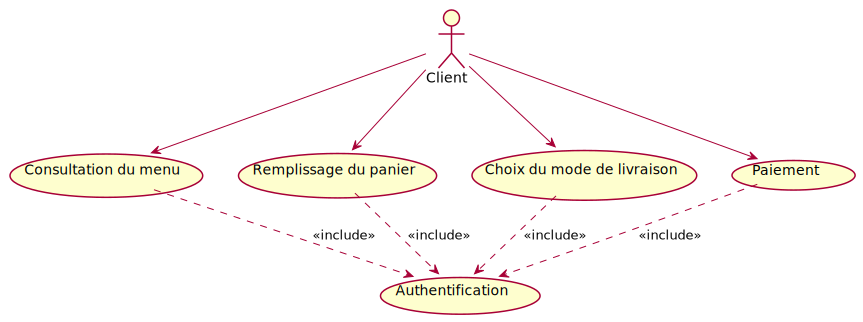
\includegraphics[width=0.9\textwidth,height=0.3\textheight]{Ressources/Client.png}
\caption{Diagramme de cas d'utilisation décrivant le rôle des clients du site}
\par
\end{centering}
\end{figure}

\clearpage



\subsubsection{Rôle des administrateurs}
Voici le diagramme de cas d'utilisation concernant le rôle des administrateurs du site.

\begin{figure}[H]
\begin{centering}
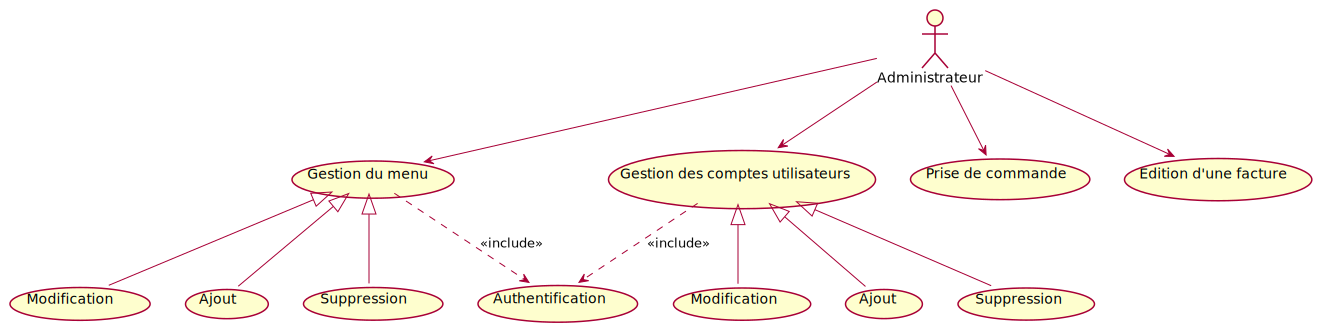
\includegraphics[width=0.95\textwidth,height=0.25\textheight]{Ressources/Administrateur.png}
\caption{Diagramme de cas d'utilisation décrivant le rôle des administrateurs du site}
\par
\end{centering}
\end{figure}

\clearpage
